\section{Introduction}
  \begin{frame}
    \frametitle{Definitions and presentation}
      \begin{itemize}
        \item \textbf{Network:} an \textbf{interconnected} group or system
        \item \textbf{Internet:} world wide \textbf{interconnected system of network\emph{s}} \color{blue}\href{http://tools.ietf.org/html/rfc791}{RFC791 (September 1981)}\color{black}
        \item \textbf{IP:} Internet \textbf{Protocol} provides the functions necessary to deliver a package of bits from a source to a destination over a network
        \item \textbf{(world wide) Web:} \textbf{network} consisting of a collection of Internet websites using HTTP
      \end{itemize}
  \end{frame}
  \begin{frame}
    \frametitle{Definitions and presentation}
      \begin{itemize}
        \item \textbf{HTTP:} Hypertext Transfer \textbf{Protocol}, application-level protocol for distributed, collaborative, hypermedia information systems \color{blue}\href{http://tools.ietf.org/html/draft-ietf-httpbis-http2-14}{draft HTTP2 (July 2014)} \color{black}
        \item \textbf{FTP:} File Transfer \textbf{Protocol} promotes sharing of files, encourages the use of remote computers \color{blue}\href{http://tools.ietf.org/html/rfc959}{RFC959 (October 1985)} \color{black}
        %\item \textbf{TCP:} Transmission Control \textbf{Protocol} is intended for use as a highly reliable host-to-host \color{blue}\href{http://tools.ietf.org/html/rfc761}{RFC761 (January 1980)} \color{black}
        %\item \textbf{UDP:} User Datagram \textbf{Protocol} provides  a procedure  for application  programs  to send messages  to other programs  with a minimum  of protocol mechanism \color{blue}\href{http://tools.ietf.org/html/rfc768}{RFC768 (August 1980)} \color{black}
        \item \textbf{RFC:} Request For Comments (Internet Draft (ID), RFC, Internet Standard)
      \end{itemize}
  \end{frame}
  \begin{frame}
    \frametitle{Definitions and presentation}
      \begin{itemize}
        \item \textbf{Router:} network \textbf{hardware} providing routing services
        \item \textbf{Routing:} \textbf{algorithm processed} to decide where to forward a packet
        \item \textbf{Forwarding:} \textbf{\emph{action}} of moving a packet from one NIC to another
        \item \textbf{NIC:} Network Interface Card
        \item \textbf{Switch (hub):} network \textbf{hardware} connecting systems using packet switching
        \item \textbf{Packet switching:} forward-like method regardless of the content (destination-based)
        \item \textbf{NAT:} Network Address Translation, router modifying IP address into another IP address (PAT).
      \end{itemize}
  \end{frame}
  \begin{frame}
    \frametitle{Definitions and presentation}
      \begin{itemize}
        \item \textbf{Node (network):} any entity that can send packets to/receive packets from a network through a NIC
        \item \textbf{Client:} \textbf{computer} able to send requests to a server
        \item \textbf{Request:} \textbf{application message} destined for a server (\emph{order})
        \item \textbf{Server:} \textbf{computer} able to respond to a client's requests
        \item \textbf{Response:} \textbf{application message} destined for a client (\emph{result})
        \item \textbf{Fat client:} \textbf{application} where most functions are processed by the client itself
        \item \textbf{Thin client:} \textbf{application} where most functions are carried out on a central server
      \end{itemize}
  \end{frame}

  \begin{frame}
    \frametitle{Network classification}
      \begin{itemize}
        \item \textbf{BAN:} Body Area Network
        \item \textbf{PAN:} Personal Area Network
        \item \textbf{(W)LAN:} (Wireless) Local Area Network (home, office, school or airport)
        \item \textbf{MAN:} Metropolitan Area Network, can cover a whole city
        \item \textbf{WAN:} Wide Area Network cover a broad area (Internet)
      \end{itemize}
  \end{frame}
  \begin{frame}
    \frametitle{Topologies}
    \begin{figure}[t]
      \centering
      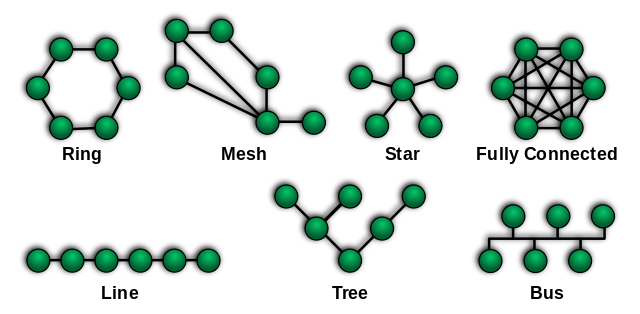
\includegraphics[height=5cm]{./imgs/topologies.png}
      \caption{\color{blue}\href{https://upload.wikimedia.org/wikipedia/commons/thumb/9/97/NetworkTopologies.svg/640px-NetworkTopologies.svg.png}{upload.wikimedia.org}}
      \label{fig:topologies}
    \end{figure}
  \end{frame}
  \begin{frame}
    \frametitle{Topologies}
    \begin{itemize}
      \item \textbf{Point-to-point:} two entities directly connected to each other (tunnel).
      \item \textbf{Ring:} data go around the ring, unidirectional way network.
      \item \textbf{Mesh:} all nodes cooperate in the distribution of data in the network\footnote{\color{blue}\href{http://www.newscientist.com/article/dn26285-hong-kong-protesters-use-a-mesh-network-to-organise.html}{Hong Kong protesters used a mesh network to organize (2014)}}.
      \item \textbf{Star:} all messages go through the same central node, reducing network failure.
      \item \textbf{Fully connected:} all nodes are connected to all other nodes.
      \item \textbf{Line:} bidirectional link between two nodes. Node can only send packet going through its neighbors.
      \item \textbf{Bus:} all nodes are connected to the same media. Only one can send a packet at a time, which all others then receive.
      \item \textbf{Tree:} hierarchical topology, such as a binary tree.
    \end{itemize}
  \end{frame}
  \begin{frame}
    \frametitle{Bonus}
    \begin{figure}[p]
      \centering
      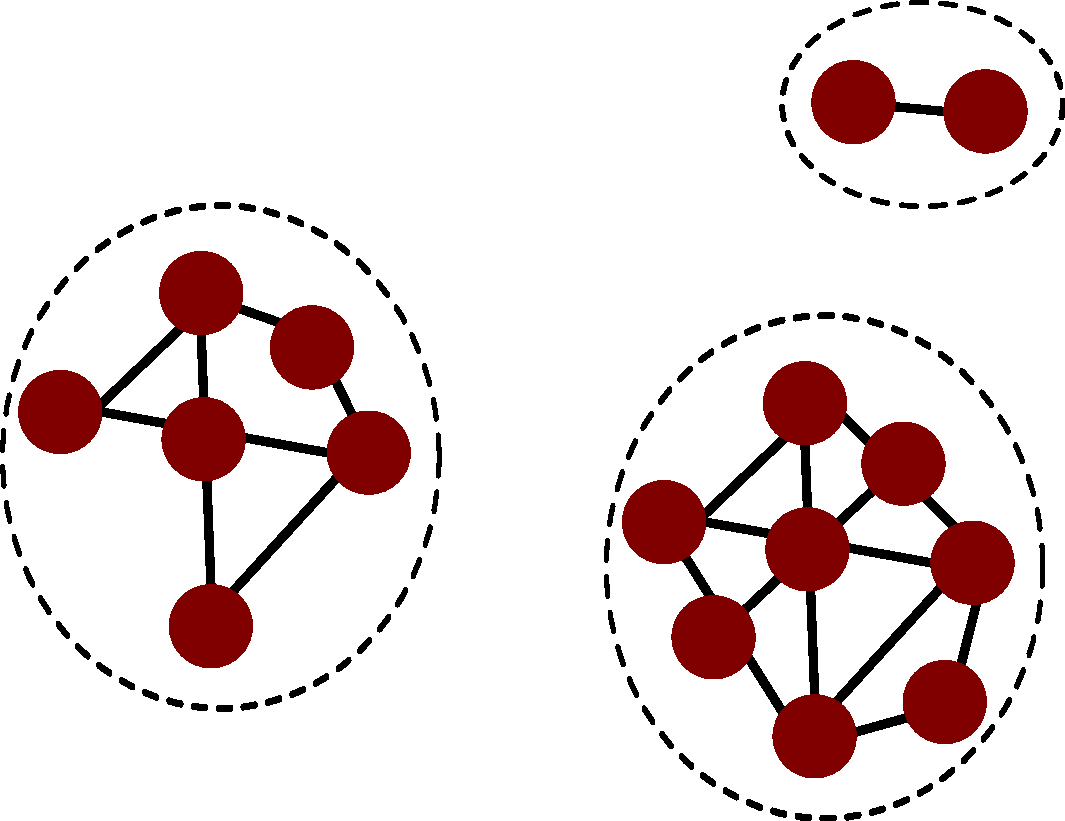
\includegraphics[height=3cm]{./imgs/dmanet.pdf}
      \caption{Disconnected MANET illustration}
      \label{fig:dmanet}
    \end{figure}
  \end{frame}
  \begin{frame}
    \frametitle{Bonus}
    \begin{figure}[p]
      \centering
      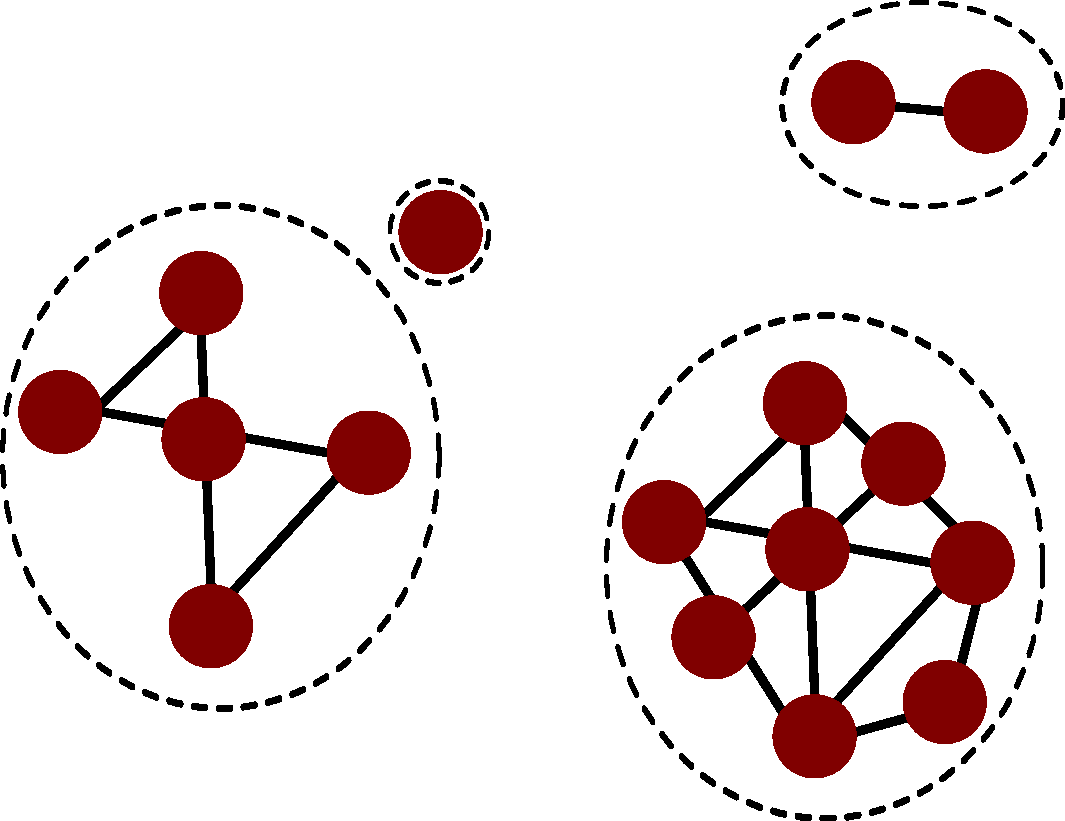
\includegraphics[height=3cm]{./imgs/store-carry-fwd-0.pdf}
      \caption{Store-carry-and-forward}
    \end{figure}
  \end{frame}
  \begin{frame}
    \frametitle{Bonus}
    \begin{figure}[p]
      \centering
      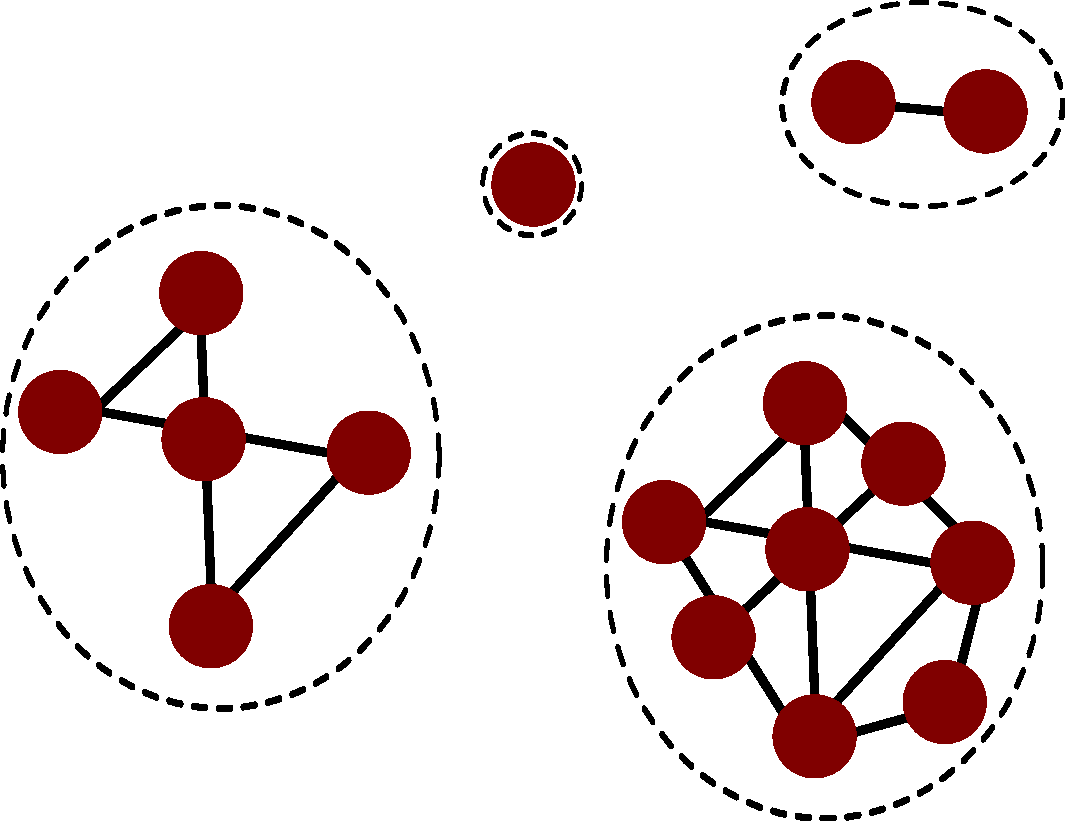
\includegraphics[height=3cm]{./imgs/store-carry-fwd-1.pdf}
      \caption{Store-carry-and-forward}
    \end{figure}
  \end{frame}
  \begin{frame}
    \frametitle{Bonus}
    \begin{figure}[p]
      \centering
      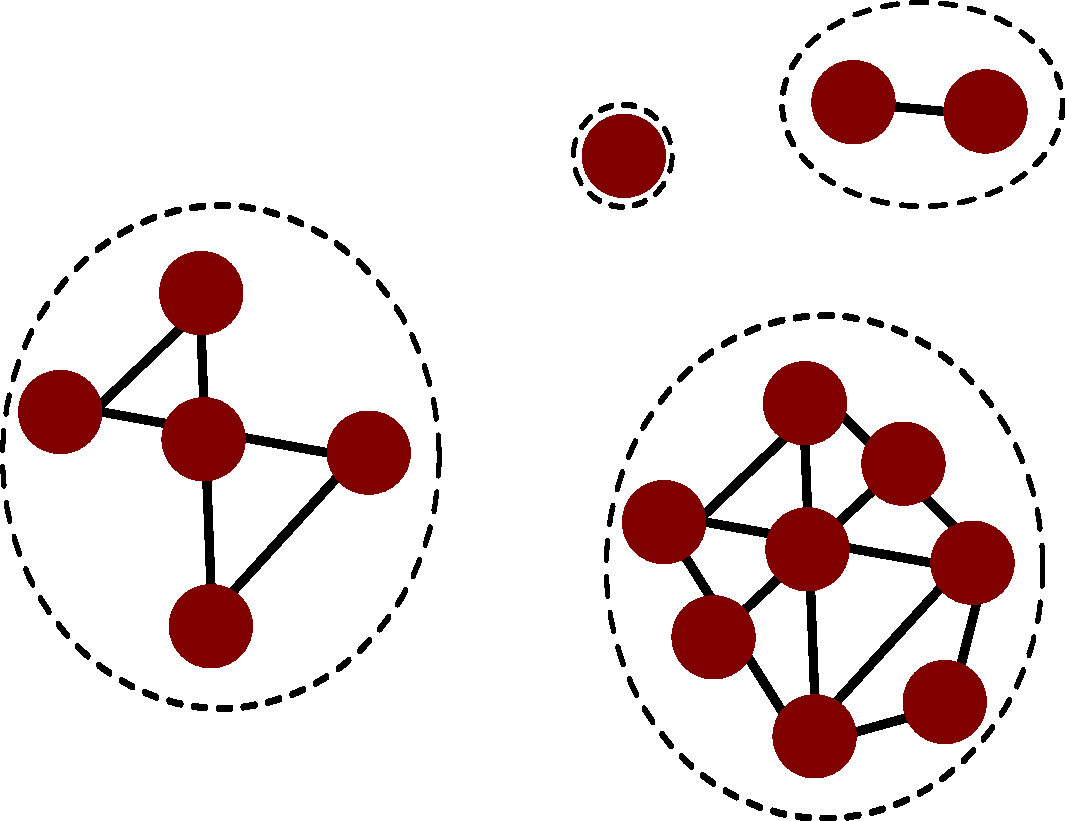
\includegraphics[height=3cm]{./imgs/store-carry-fwd-2.pdf}
      \caption{Store-carry-and-forward}
    \end{figure}
  \end{frame}
  \begin{frame}
    \frametitle{Bonus}
    \begin{figure}[p]
      \centering
      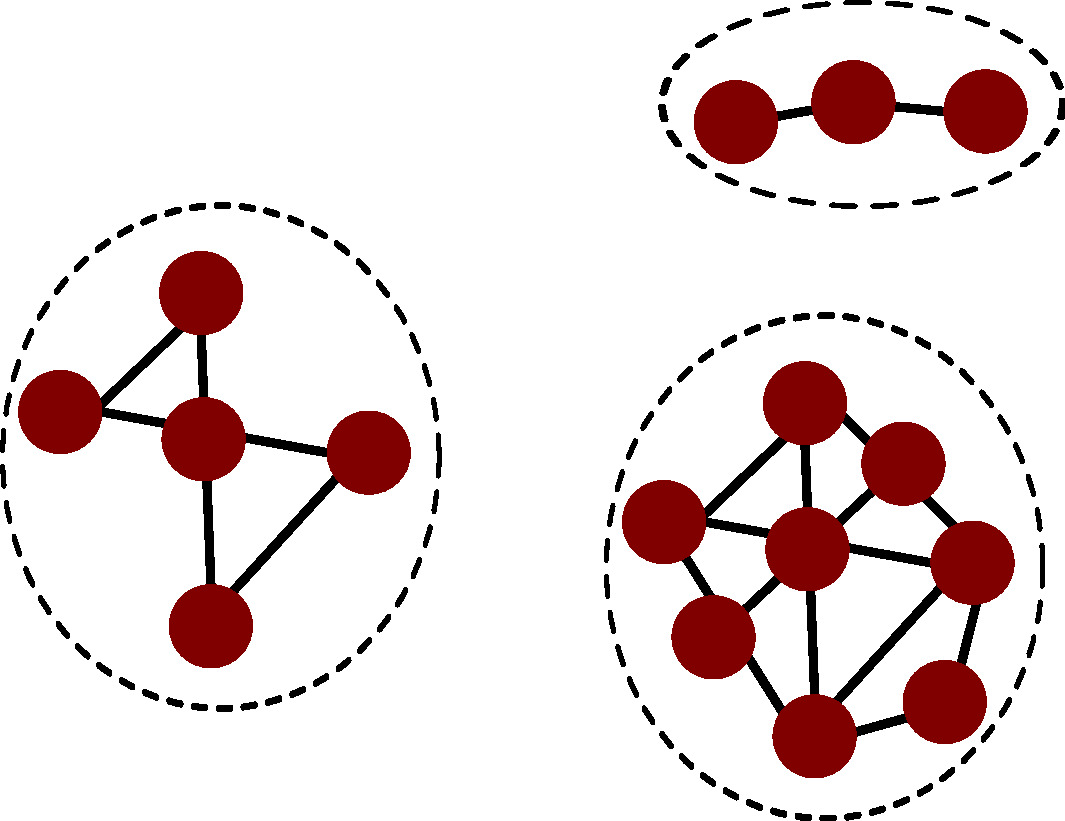
\includegraphics[height=3cm]{./imgs/store-carry-fwd-3.pdf}
      \caption{Store-carry-and-forward}
    \end{figure}
  \end{frame}


\begin{frame}
    \frametitle{HTTP request/response example}
      Enter \color{blue}\href{http://getbootstrap.com}{getbootstrap.com} \color{black} in your browser\pause
      \begin{figure}
    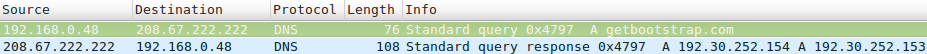
\includegraphics[width=11.5cm]{./imgs/dns-req.png}
  \caption{DNS request/response}
      \end{figure}
      \pause
      \begin{figure}
    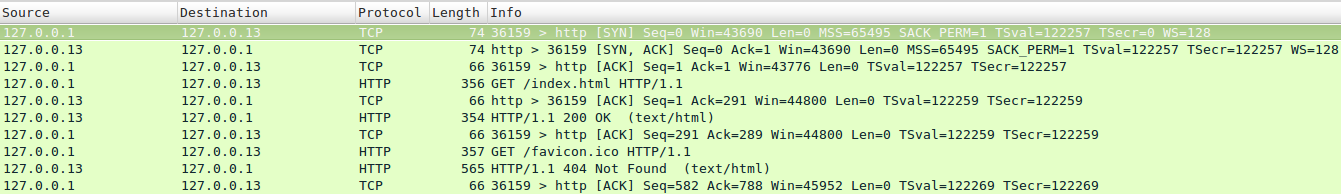
\includegraphics[trim = 0 0 100mm 0, clip, width=11.5cm]{./imgs/http-req.png}
  \caption{HTTP request/response}
      \end{figure}
  \end{frame}
  \begin{frame}
    \frametitle{To read}
      {\color{blue} \href{https://github.com/alex/what-happens-when}{https://github.com/alex/what-happens-when}}
      \begin{itemize}
          \item DNS lookup
          \item ARP process
          \item Opening of a socket
          \item TLS handshake
          \item HTTP protocol
          \item HTTP Server Request Handle
      \end{itemize}
  \end{frame}
  \begin{frame}
    \frametitle{How do messages reach their destination?}
      \begin{figure}
    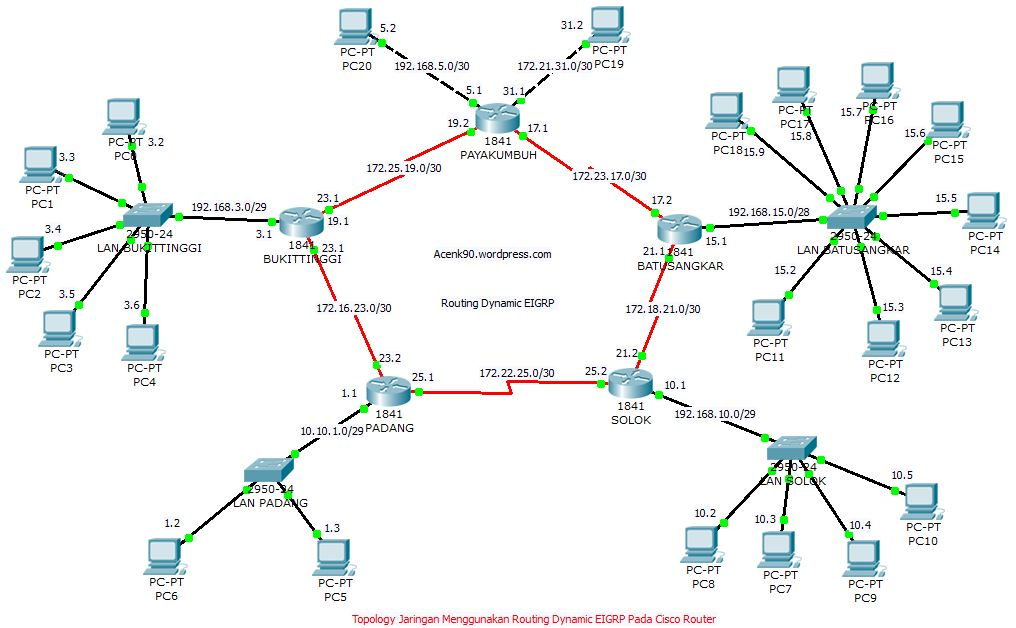
\includegraphics[width=9.5cm]{./imgs/routing.jpg}
  \caption{\color{blue}\href{http://acenk90.files.wordpress.com}{acenk90.files.wordpress.com}}
  \label{fig:routing}
      \end{figure}
  \end{frame}
    \begin{frame}
    \frametitle{More like this...}
      \begin{figure}
    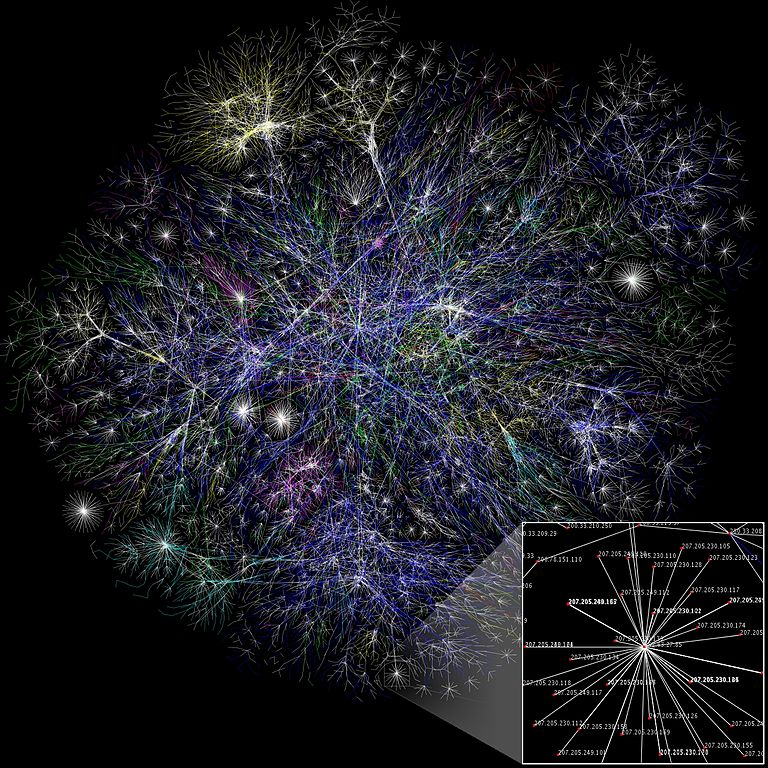
\includegraphics[height=6.5cm]{./imgs/map.jpg}
  \caption{\color{blue}\href{https://upload.wikimedia.org/wikipedia/commons/thumb/d/d2/Internet_map_1024.jpg/768px-Internet_map_1024.jpg}{wikimedia.org}}
  \label{fig:map}
      \end{figure}
  \end{frame}

  \begin{frame}
    \frametitle{Models overview (OSI and TCP/IP)}
    \begin{figure}[t]
      \centering
      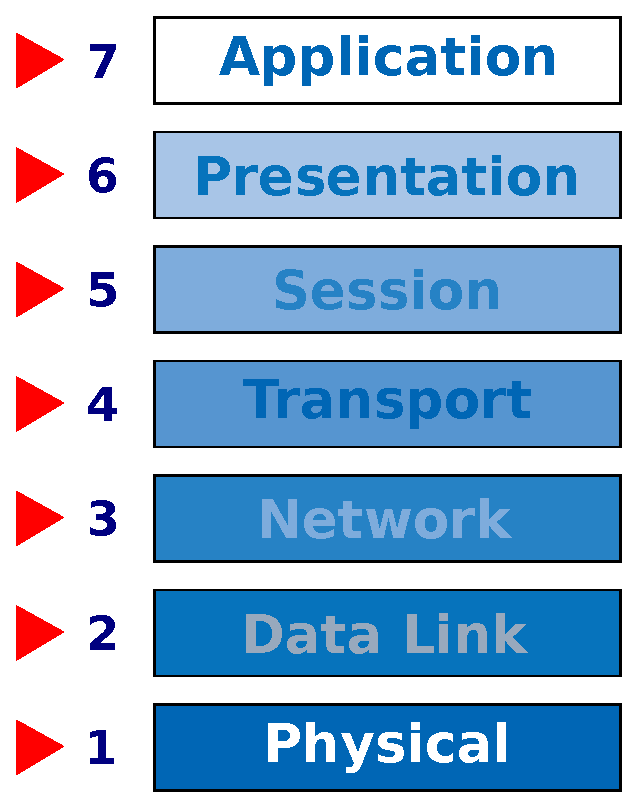
\includegraphics[height=6cm]{./imgs/osi_model.eps}
      \caption{OSI model}
      \label{fig:osi_mod}
    \end{figure}
  \end{frame}
  \begin{frame}
    \frametitle{N\textsuperscript{th} layer communicate with N\textsuperscript{th} layer..}
    \begin{figure}[t]
      \centering
      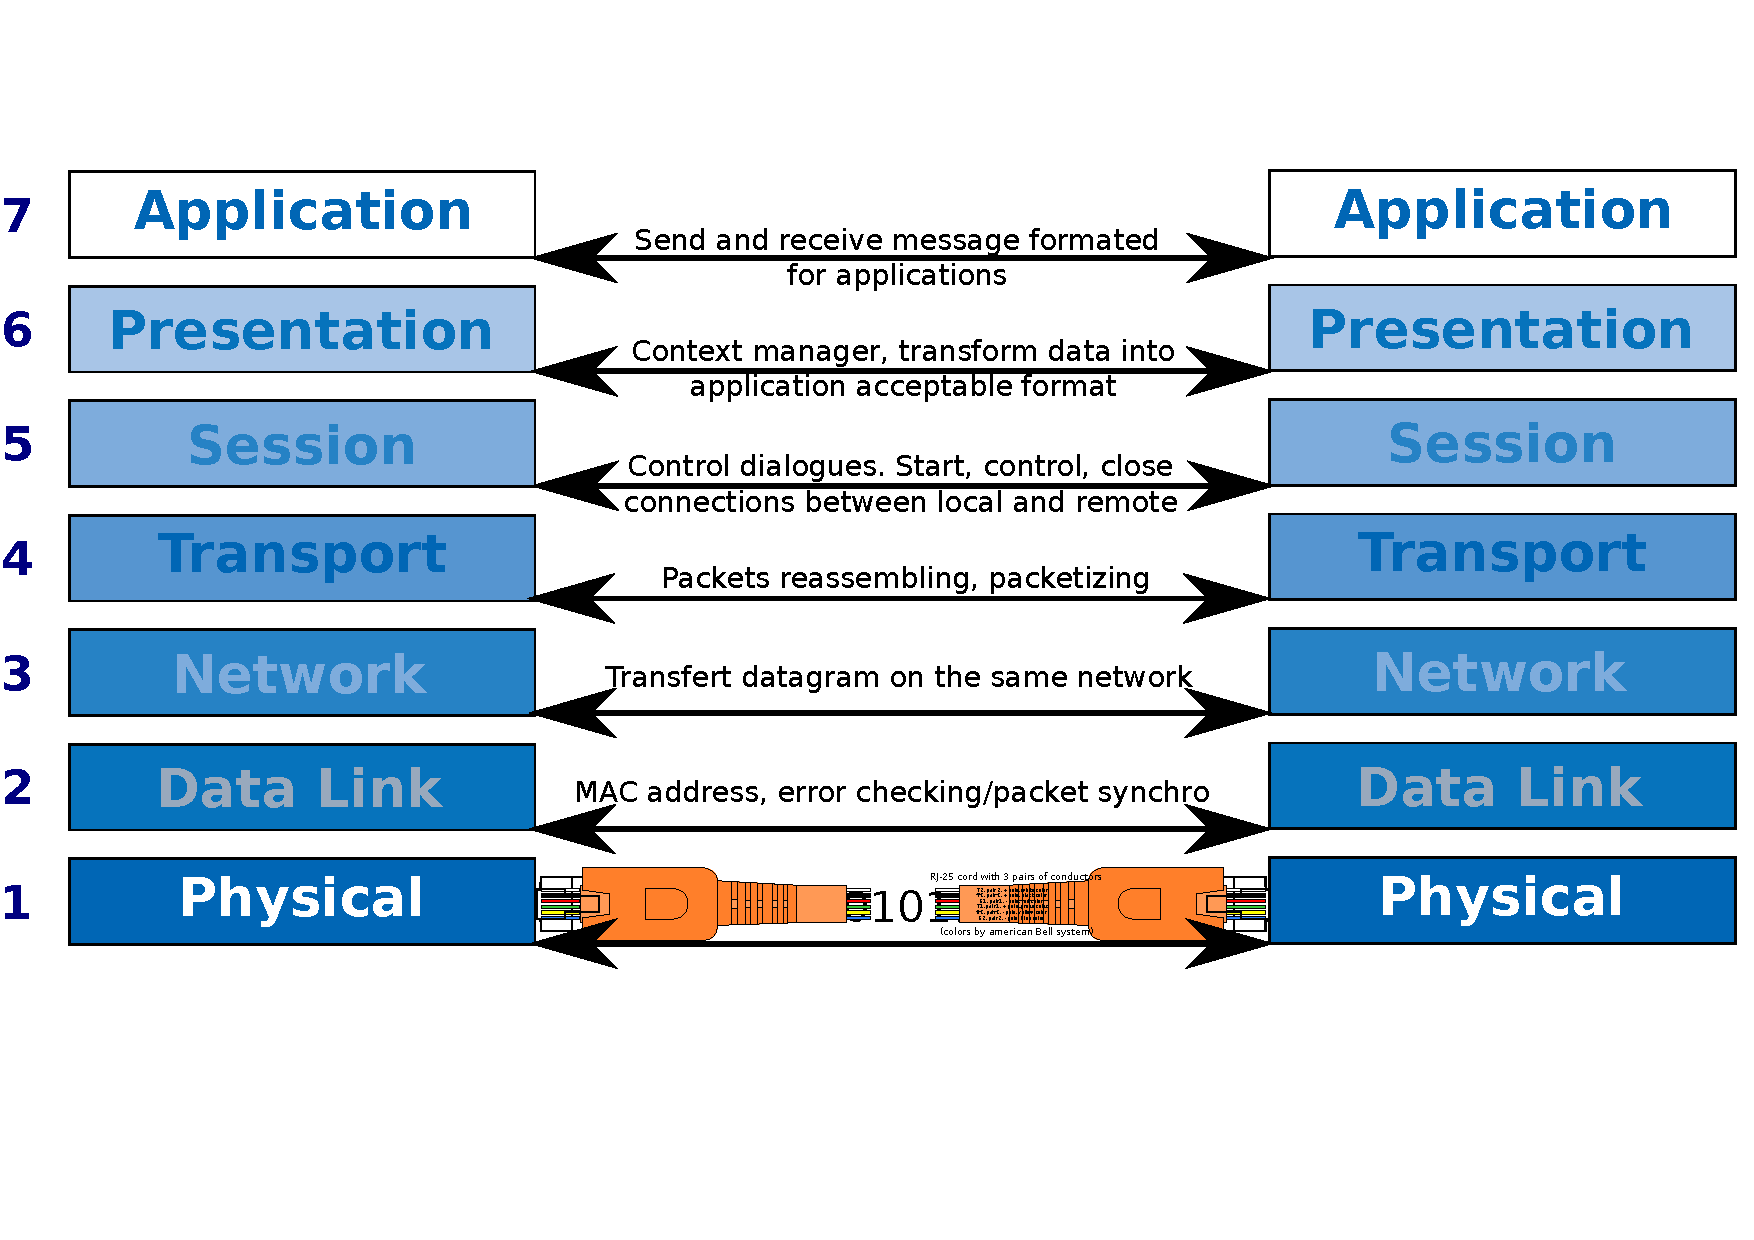
\includegraphics[height=7.5cm]{./imgs/layer2layer.pdf}
      \caption{layer to layer}
      \label{fig:layer2layer}
    \end{figure}
  \end{frame}
  \begin{frame}
    \frametitle{.. thanks to 3-\textsuperscript{th} layers}
    \begin{figure}[t]
      \centering
      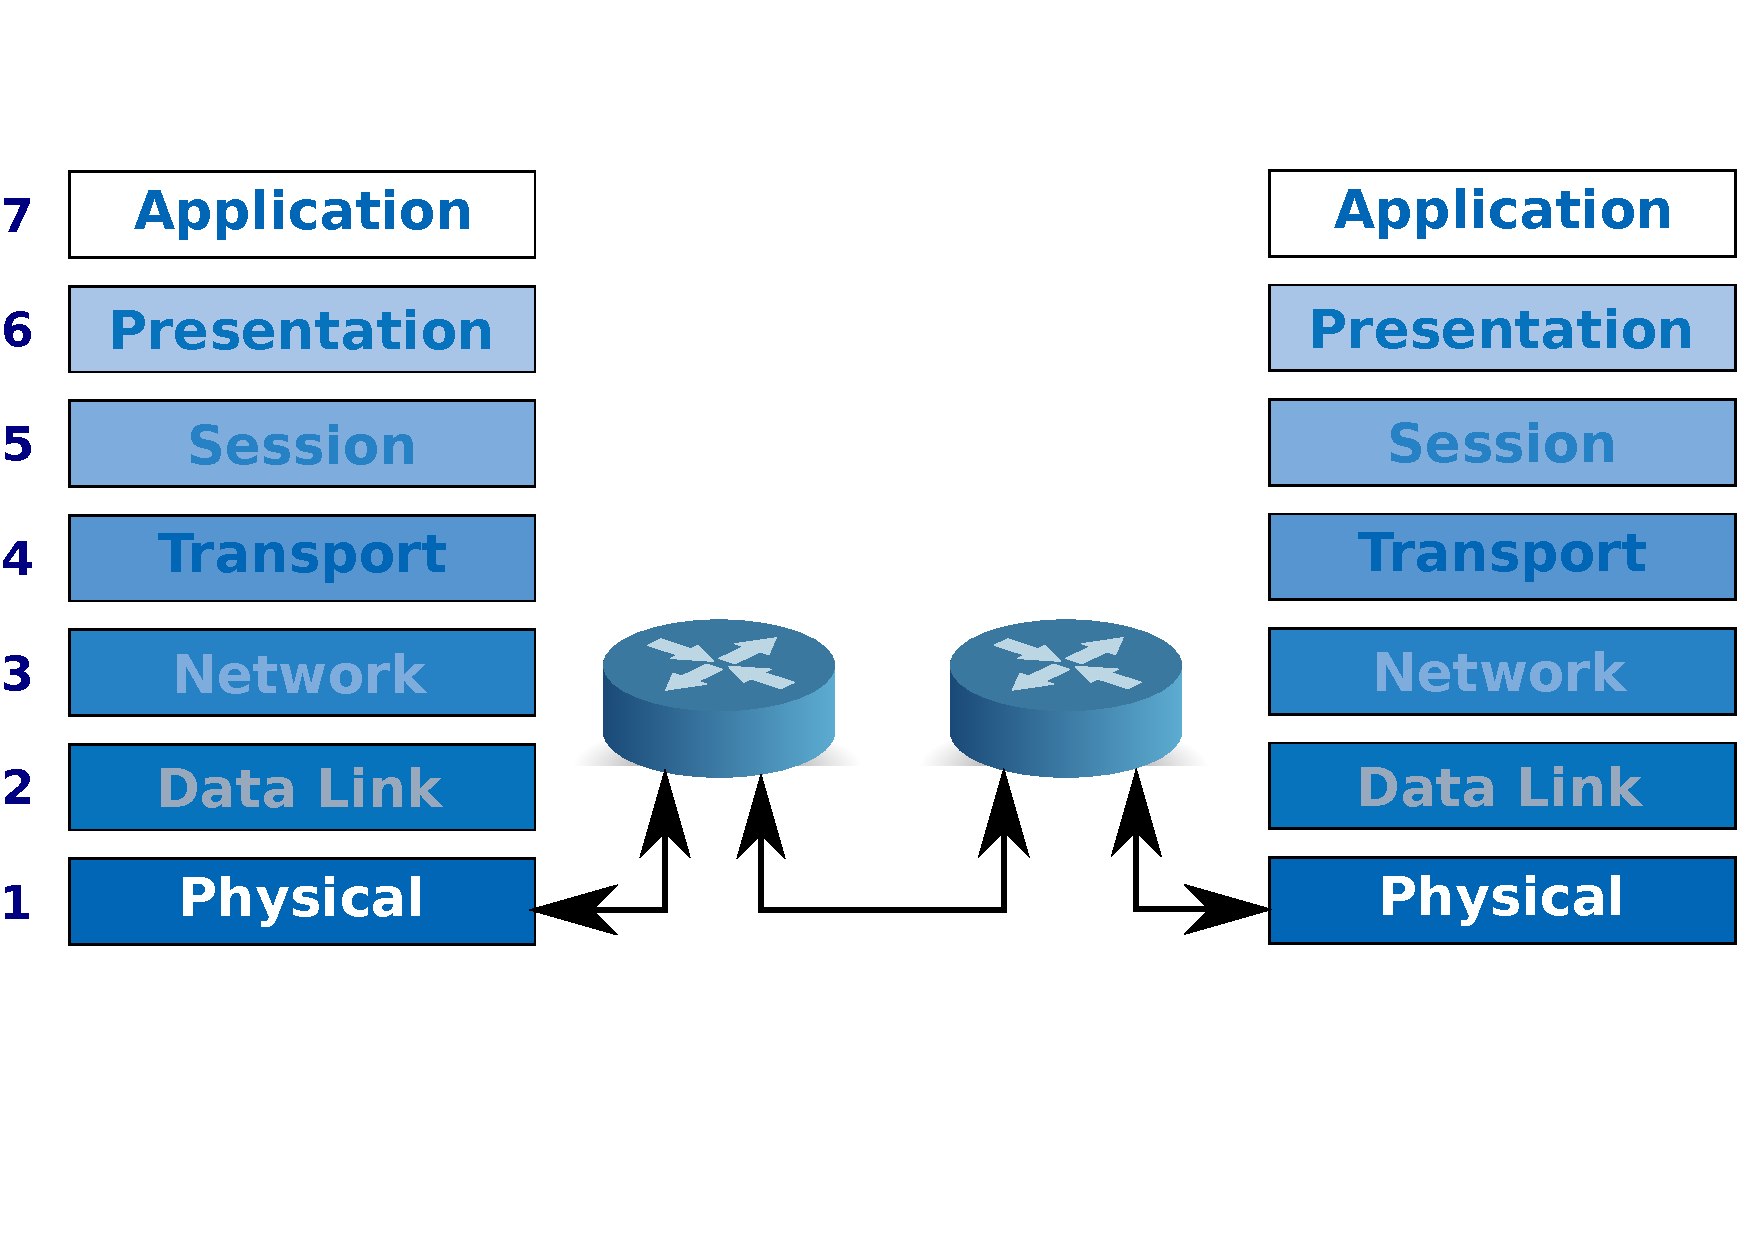
\includegraphics[height=7.5cm]{./imgs/layers_routers.pdf}
      \caption{layers and routing}
      \label{fig:layers_routing}
    \end{figure}
  \end{frame}
  \begin{frame}
    \frametitle{One single protocol, one single layer}
    \begin{figure}[t]
      \centering
      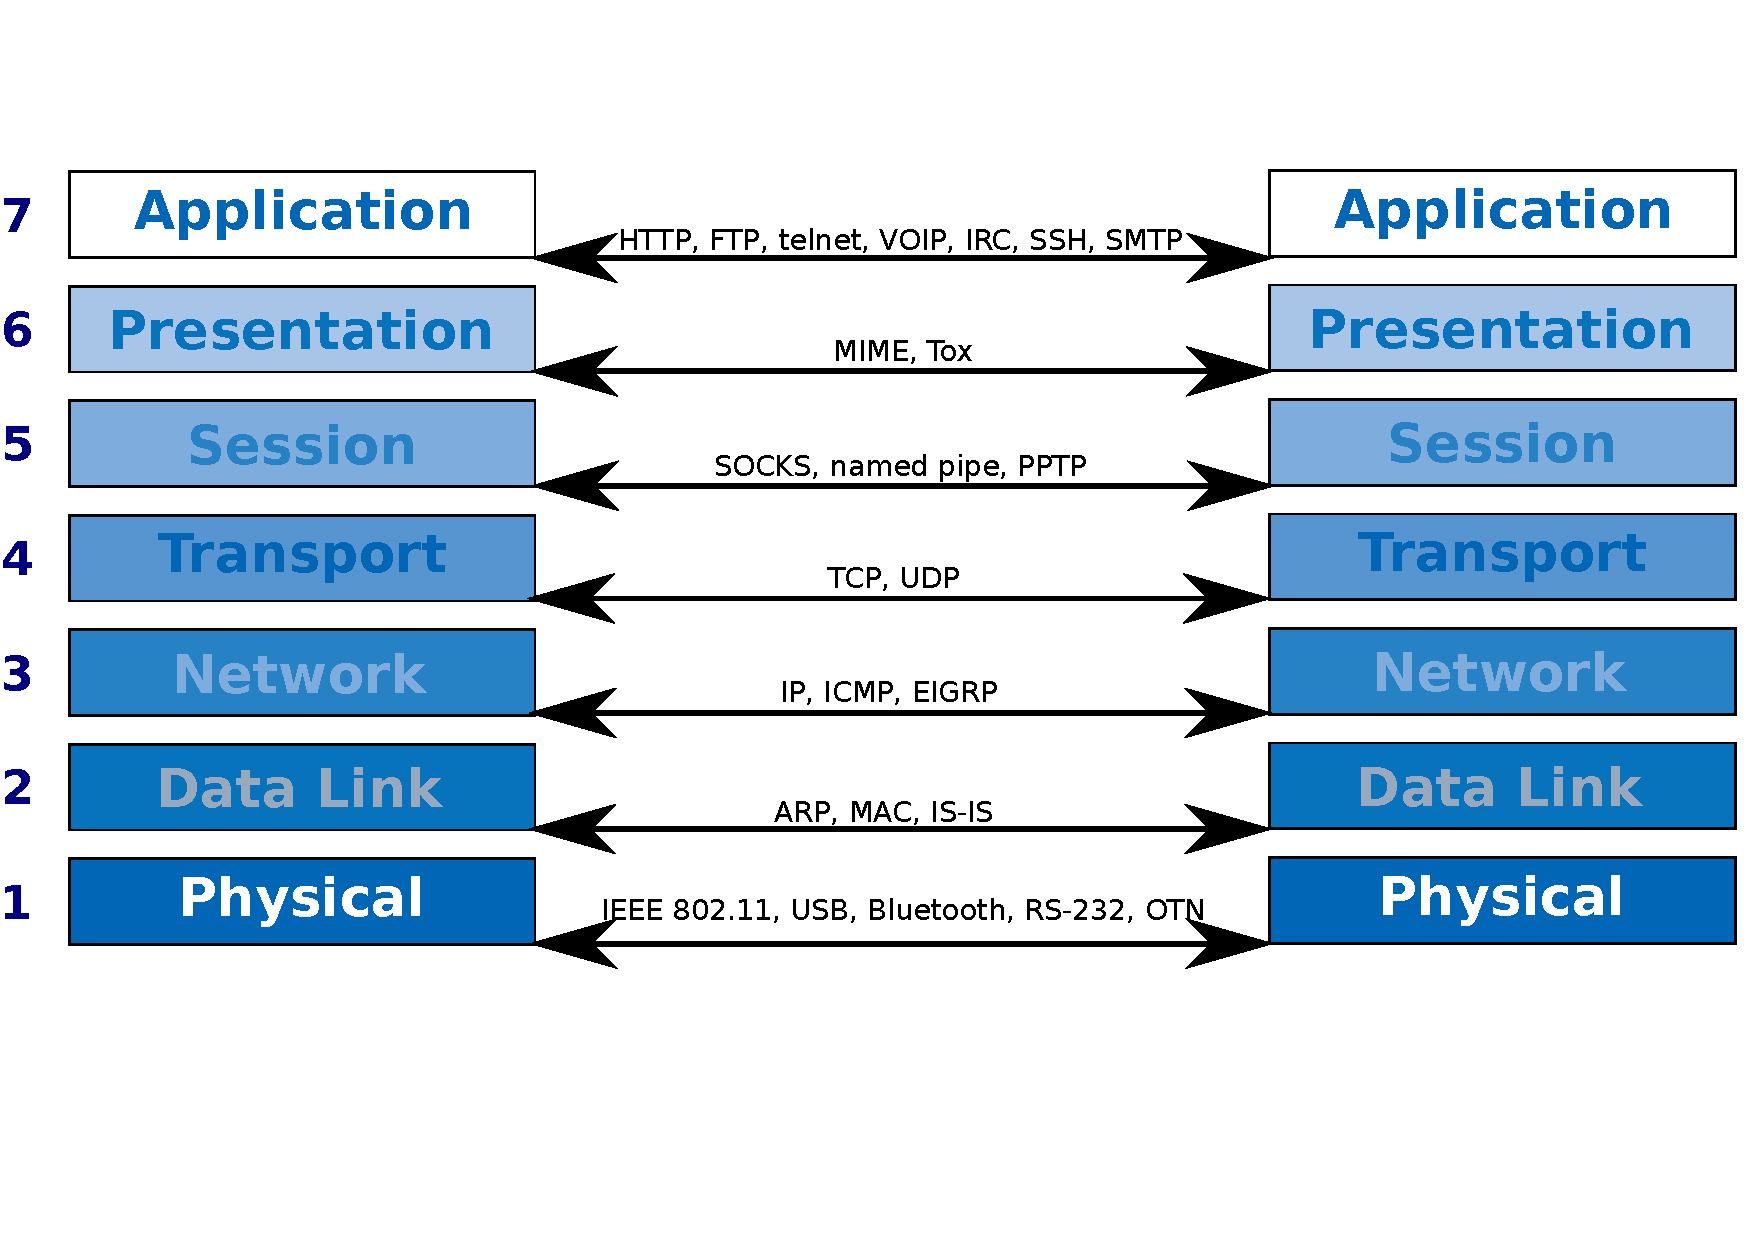
\includegraphics[height=7.5cm]{./imgs/layer2protocol.pdf}
      \caption{protocols and layers}
      \label{fig:layers2proto}
    \end{figure}
  \end{frame}
  \begin{frame}
    \frametitle{Encapsulation}
    \begin{figure}[t]
      \centering
      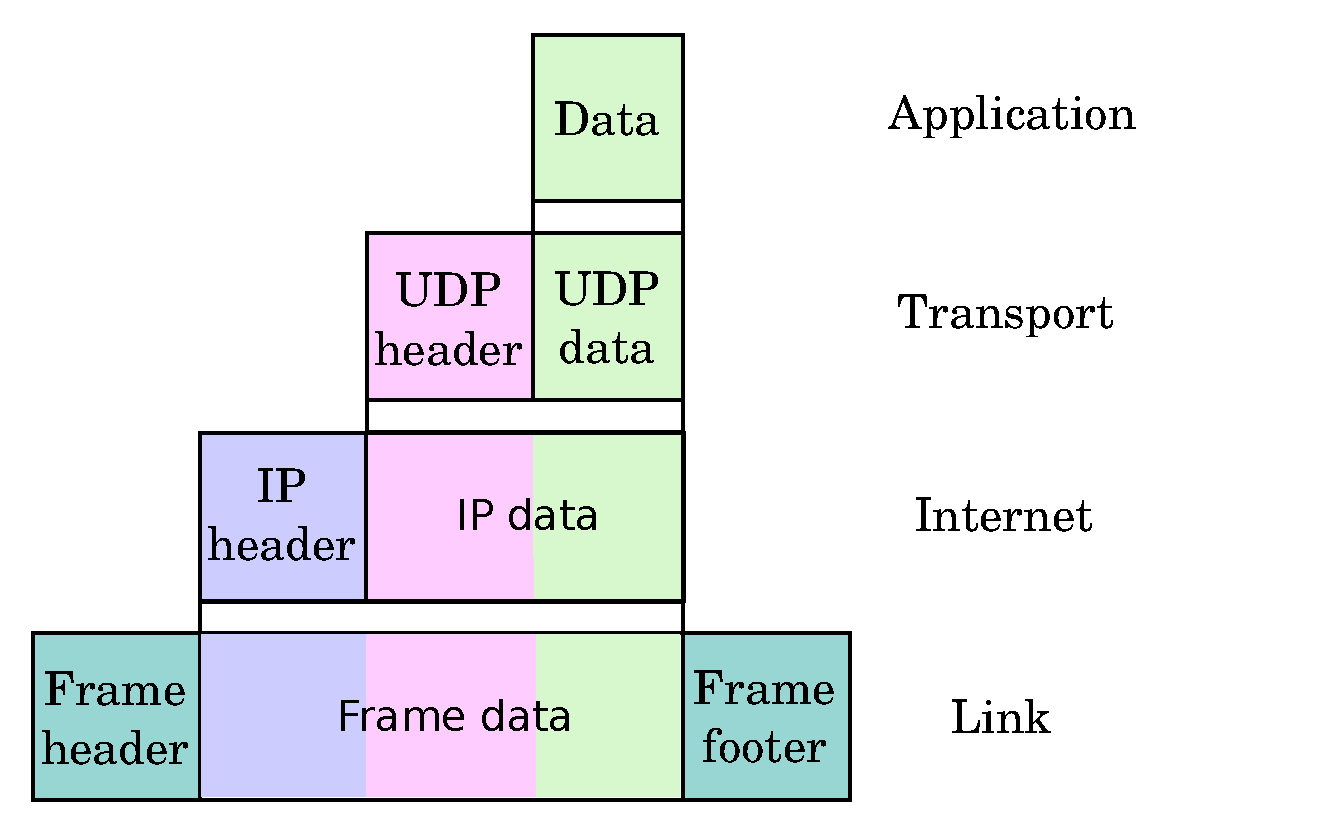
\includegraphics[height=5cm]{./imgs/encapsulation.pdf}
      \caption{Encapsulation}
      \label{fig:encapsulation}
    \end{figure}
  \end{frame}

  \begin{frame}
    \frametitle{Reading}
    \begin{block}{Reading list:}
      \begin{itemize}
        \item "Computer Networks" by A Tanenbaum, Andrew S., G ISBN 013162959X
        \item http://nmap.org/book/toc.html
        \item http://blog.nodenexus.com/2014/11/28/a-shark-on-the-network/
        \item and many many other resources on the Internet freely available\footnote{{\color{blue}\href{http://intronetworks.cs.luc.edu/current/ComputerNetworks.pdf}{An Introduction to Computer Networks (21: Security)}} by Peter L Dordal}! If you can read it, knowledge is reachable\footnote{such as this {\color{blue}\href{https://silverskylabs.github.io/yakhak/}{example of Wireshark using}} or {\color{blue}\href{https://github.com/alex/what-happens-when}{what-happens-when}}}!
      \end{itemize}
    \end{block}
  \end{frame}

  \begin{frame}
    \frametitle{Whatching}
    \begin{block}{Watching list:}
      \begin{itemize}
        \item DEF CON 22 Hacking Conference Presentation By Christopher Soghoian - Blinding The Surveillance State
        \footnote{{\color{blue}\href{https://media.defcon.org/DEF CON 22/DEF CON 22 video and slides/}{media.defcon.org}}}
        \item any other defcon
        \item Mr Robot, that's a good serie!
      \end{itemize}
    \end{block}
  \end{frame}
